% Auto-generated from diplom_asp/content/hierarchical_safe_exploration.tex
\chapter{Решение проблемы безопасного исследования с помощью иерархической структуры}
\label{ch:hierarchical_safe_exploration}

В предыдущей главе рассматривалось использование модели мира для оценки последствий действий до их выполнения. Такой подход полезен для безопасного планирования, однако он плохо масштабируется на задачи с большим горизонтом. Чем длиннее требуется траектория, тем сильнее накапливается ошибка модели, и тем менее надёжной становится оценка всей последовательности действий.

Данная глава посвящена решению этой проблемы с помощью иерархической структуры (рис.~\ref{fig:sgsafe_idea}). Основная идея состоит в том, что вместо прямого поиска траектории к удалённой цели агент использует промежуточные подцели, которые направляют исследование среды. В методе SG-Safe~\cite{gorbov2026sgsafe} стратегия генерации подцелей применяется на этапе обучения и помогает безопасной стратегии находить более информативные области пространства состояний. При этом подцели не являются жёсткими командами, обязательными для точного достижения, а используются как дополнительный обучающий сигнал. На этапе исполнения применяется только обученная безопасная стратегия, что позволяет избежать дополнительных затрат на планирование.

\begin{figure}[t]
    \centering
    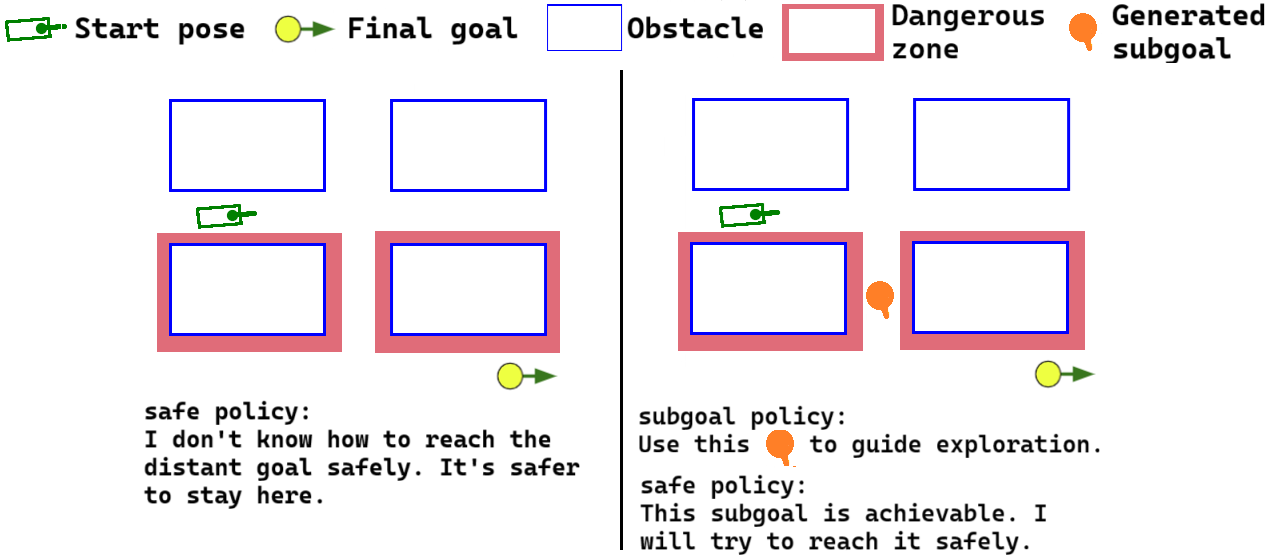
\includegraphics[width=\linewidth]{article_idea_env.png}
    \caption{Безопасное исследование с использованием подцелей. \textbf{Слева}: одноуровневая безопасная стратегия может не находить траекторию к удалённой цели. \textbf{Справа}: промежуточные подцели направляют исследование и упрощают достижение цели.}
    \label{fig:sgsafe_idea}
\end{figure}

В задачах с большим горизонтом агент получает значимую награду только после выполнения длинной последовательности действий. Примерами являются навигация вокруг препятствий, прохождение коридоров, манипуляция объектами и достижение удалённых целей. В задачах с большим горизонтом эта проблема проявляется особенно заметно. Чтобы найти траекторию к цели, агенту нужно выходить за пределы уже известных безопасных действий. Однако именно такие попытки чаще всего и приводят к посещению опасных состояний или накоплению штрафов нарушений.

\section{Метод SG-Safe}
\label{subsec:sgsafe}

В SG-Safe безопасная стратегия обучается вместе со стратегией генерации подцелей. Безопасная стратегия выбирает действия с учётом награды и штрафов нарушений, а генератор подцелей используется для того, чтобы направлять обучение в задачах с длинным горизонтом. Вместо прямого поиска полной траектории к конечной цели агент получает промежуточные состояния, которые делают исследование более управляемым. Безопасная стратегия обучается с использованием лагранжевой целевой функции, что позволяет максимизировать возврат по задаче и одновременно штрафовать нарушения безопасности. Как показано на рис.~\ref{fig:sgsafe_method_scheme}, SG-Safe чередует две основные процедуры: 1)~сбор опыта безопасной стратегией и сохранение траекторий в буфере HER с переиспользованием опыта и подстановкой достигнутых целей; 2)~обновление безопасной стратегии с использованием подцелей, сгенерированных на основе переходов из буфера. Такая схема повышает эффективность обучения в задачах с разреженной наградой и большим горизонтом.

\subsection{Безопасная стратегия метода SG-Safe}
\label{subsec:sgsafe_safe_policy}

\begin{figure}[t]
    \centering
    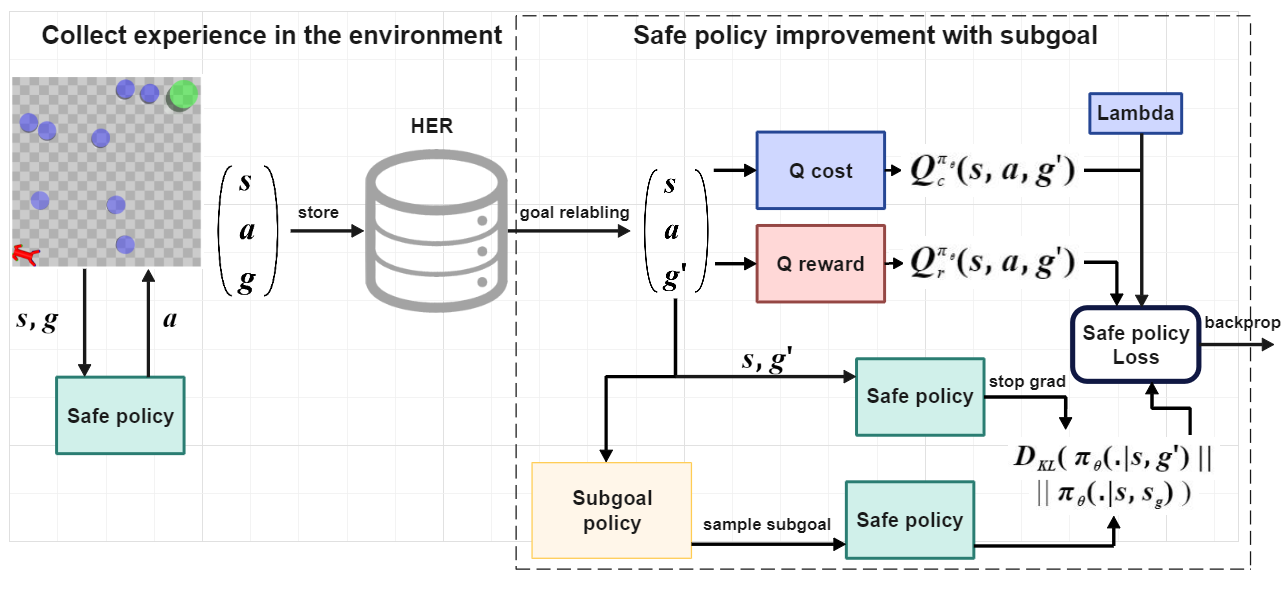
\includegraphics[width=0.95\textwidth]{method_scheme_3.png}
    \caption{Схема метода SG-Safe. Метод включает сбор опыта безопасной стратегией с сохранением траекторий в HER buffer и последующее улучшение безопасной стратегии с использованием промежуточных подцелей.}
    \label{fig:sgsafe_method_scheme}
\end{figure}

Одним из распространённых подходов к решению марковских процессов принятия решений с ограничениями являются методы на основе функции лагранжиана, которые часто комбинируются с внеполитическим градиентным алгоритмом SAC. Подход на основе функции лагранжиана сводит задачу оптимизации с ограничениями к безусловной задаче оптимизации с помощью множителей Лагранжа $\lambda_i$, задающих веса ограничений безопасности. Эти множители штрафуют нарушения ограничений, учитывая расхождение между допустимым бюджетом штрафов $d_i$ и ожидаемой дисконтированными штрафами $C_i(\pi)$. В данной работе рассматривается случай одного ограничения безопасности, поэтому далее используется один множитель Лагранжа $\lambda_i = \lambda$, один бюджет штрафов $d_i = d$ и одна дисконтированные штрафы $C_i(\pi) = C(\pi)$.

Для награды и штрафов обучаются две $Q$-функции: $Q^{\pi_\theta}_r$ для оценки награды и $Q^{\pi_\theta}_c$ для оценки штрафов. Они минимизируют ошибки Беллмана с учётом энтропии:
\begin{equation}
\left(
Q^{\pi_\theta}_r(s_t,a_t)
-
\left(
r(s_t,a_t)
+
\gamma Q^{\pi_\theta}_r(s_{t+1},a_{t+1})
-
\alpha \log \pi_\theta(a_{t+1}|s_{t+1})
\right)
\right)^2,
\end{equation}
\begin{equation}
\left(
Q^{\pi_\theta}_c(s_t,a_t)
-
\left(
c(s_t,a_t)
+
\gamma Q^{\pi_\theta}_c(s_{t+1},a_{t+1})
-
\alpha' \log \pi_\theta(a_{t+1}|s_{t+1})
\right)
\right)^2,
\end{equation}
где $a_{t+1} \sim \pi(a_{t+1}|s_{t+1})$.

Стратегия оптимизируется путём минимизации следующей лагранжевой функции:
\begin{equation}
\label{eq:sgsafe_sac_lagrangian}
L(\theta,\lambda)=
\mathbb{E}\Big[
\alpha' \log \pi_{\theta}(a_t|s_t)
-
Q^{\pi_\theta}_r(s_t,a_t)
+
\lambda Q^{\pi_\theta}_c(s_t,a_t)
\Big].
\end{equation}

Множитель Лагранжа $\lambda$ обучается адаптивно за счёт минимизации функции потерь:
\begin{equation}
\label{eq:sgsafe_multiplier_optimization}
J_s(\lambda)=
\mathbb{E}\Big[\lambda\big(Q^{\pi_\theta}_c(s_t,a_t)-d\big)\Big].
\end{equation}

Такое правило обновления уменьшает вес безопасности $\lambda$, когда ограничение выполняется, то есть $Q^{\pi_\theta}_c(s_t,a_t) \leq d$, и увеличивает его при нарушении ограничения. В результате при превышении допустимого бюджета штрафов оптимизация стратегии сильнее штрафует небезопасные действия.

В реализации для критиков награды и штрафов используются парные $Q$-функции: $\{Q_{r,1}, Q_{r,2}\}$ и $\{Q_{c,1}, Q_{c,2}\}$. При вычислении целевых значений Беллмана берётся минимум по соответствующим целевым критикам, что снижает переоценку значений. Целевые сети для всех критиков обновляются с помощью полиномиального усреднения с коэффициентом $\tau = 0.005$. Следующее действие $a_{t+1}$ выбирается текущей стратегией $\pi_\theta$, а целевое значение включает стандартный энтропийный член SAC: $-\alpha' \log \pi_\theta(a_{t+1}\mid s_{t+1})$. Температура энтропии $\alpha' = 0.1$ рассматривается как фиксированный гиперпараметр.

\subsection{Стратегия генерации подцелей}
\label{subsec:sgsafe_subgoal_policy}

Стратегия генерации подцелей используется для повышения эффективности обучения в задачах с большим горизонтом. Она генерирует промежуточные подцели между начальным состоянием и конечной целью, тем самым направляя низкоуровневую стратегию к достижимым и информативным состояниям. В основе данного компонента лежит подход RIS, включающий стратегию генерации подцелей и низкоуровневую стратегию. Стратегия генерации подцелей формирует достижимые подцели и при этом сохраняет согласованность с распределением состояний, которые агент способен посещать, за счёт ограничения на дивергенцию Кульбака--Лейблера.

Стратегия генерации подцелей $\pi^H$ выбирает такие подцели, которые уменьшают максимальную сложность перехода либо от текущего состояния к подцели, либо от подцели к конечной цели. Пусть $V^{\pi_\theta}$ обозначает функцию ценности, оценивающую ожидаемую дисконтированную награду. Тогда для подцели $s_g$ вводится величина
\begin{equation}
\psi_{\pi_\theta}(s_g|s,g)
    =
    \max\left(
\left|V^{\pi_\theta}(s,s_g)\right|,
\left|V^{\pi_\theta}(s_g,g)\right|
    \right).
\end{equation}
Она оценивает, насколько сложно достичь подцели из текущего состояния и затем достичь конечной цели из этой подцели.

Обновление стратегии генерации подцелей выполняется при ограничении относительно распределения посещаемых состояний $p_s$:
\begin{equation}
\label{eq:sgsafe_subgoal_policy_improvement}
\pi^H
=
\arg\max
\mathbb{E}
\left[
A^{\pi^H_k}(s_g|s,g)
\right],
\quad
\text{s.t.}
\quad
D_{\mathrm{KL}}
\left(
\pi^H(\cdot|s,g)\,\|\,p_s(\cdot)
\right)
\leq \epsilon.
\end{equation}
Здесь функция преимущества определяется как
\begin{equation}
A^{\pi^H_k}(s_g|s,g)
=
\mathbb{E}
\left[
\psi_{\pi_\theta}(s|s,g)
-
\psi_{\pi_\theta}(s_g|s,g)
\right],
\end{equation}
и измеряет ожидаемое улучшение при использовании выбранной подцели.

Для обучения низкоуровневой стратегии для каждого перехода выбирается подцель $s_g \sim \pi^H$. Затем низкоуровневая стратегия оптимизируется так, чтобы максимизировать значение функции полезности и одновременно уменьшать расхождение между распределением действий при условии конечной цели и распределением действий при условии подцели:
\begin{equation}
\pi_\theta
=
\arg\max
\mathbb{E}
\left[
Q_r^{\pi_\theta}(s,a,g)
-
\alpha
D_{\mathrm{KL}}
\left(
\pi_\theta(\cdot|s,g)\,\|\,\pi_\theta(\cdot|s,s_g)
\right)
\right].
\end{equation}
Таким образом, подцели направляют низкоуровневую стратегию к промежуточным состояниям, но при этом не заменяют исходную цель задачи.

\begin{algorithm}[t]
\caption{SG-Safe}
\label{alg:sgsafe}
\begin{algorithmic}[1]
    \State Инициализировать буфер HER $D$
    \State Инициализировать $Q^{\pi_\theta}_r$, $Q^{\pi_\theta}_c$, $\pi_{\theta}$, $\lambda$, $\pi^H$
    \For{$k = 1, 2, \ldots$}
        \State Собрать опыт в среде с помощью стратегии $\pi_\theta$ и сохранить его в $D$
        \State Выбрать мини-пакет переходов $(s_t, a_t, r_t, c_t, s_{t+1}, g) \sim D$
        \State Выбрать мини-пакет кандидатов подцелей $s'_g \sim D$
        \State Обновить $Q^{\pi_\theta}_r$ и $Q^{\pi_\theta}_c$ с использованием ошибок Беллмана с учётом энтропии
        \State Обновить множитель Лагранжа $\lambda$
        \State Обновить стратегию генерации подцелей $\pi^H$
        \State Обновить безопасную стратегию $\pi_{\theta}$ с использованием подцелей
    \EndFor
\end{algorithmic}
\end{algorithm}

\subsection{Обновление безопасной стратегии с подцелями}
\label{subsec:sgsafe_policy_update}

SG-Safe объединяет генерацию подцелей с оптимизацией стратегии при ограничениях безопасности для решения задач безопасного исследования с большим горизонтом. Во время обучения подцели направляют исследование среды, а на этапе исполнения используется только обученная безопасная стратегия.

Модифицированная целевая функция безопасной стратегии учитывает как награду за выполнение задачи, так и ограничения безопасности:
\begin{equation}
\label{eq:sgsafe_safe_policy_improvement}
\begin{split}
J(\pi_{\theta}) =\ &
\mathbb{E}_{(s,g)\sim D}
\mathbb{E}_{a\sim \pi_{\theta}(\cdot|s,g)}
\Big[
Q^{\pi_{\theta}}_{r}(s,a,g)
- \lambda Q^{\pi_{\theta}}_{c}(s,a,g) \\
& \quad - \alpha
D_{\mathrm{KL}}
\left(
\pi_{\theta}(\cdot|s,g)
\,\|\,
\pi_{\theta}(\cdot|s,s_g)
\right)
\Big].
\end{split}
\end{equation}
Здесь $Q_r^{\pi_\theta}$ отвечает за максимизацию награды, $Q_c^{\pi_\theta}$ штрафует нарушения безопасности, а член с дивергенцией Кульбака--Лейблера направляет стратегию к действиям, согласованным с сгенерированной подцелью. Обозначение $D$ соответствует буферу HER.

Сначала опыт собирается в среде только с помощью безопасной стратегии $\pi_\theta(\cdot|s,g)$ и сохраняется в буфер HER. Для улучшения сходимости в задачах с разреженной наградой в буфере HER неуспешные эпизоды переиспользуются с подстановкой достигнутых целей. Это позволяет получать более частые обучающие сигналы и повышает устойчивость обучения.

Далее из буфера HER выбираются мини-пакеты переходов, по которым обновляются критик награды $Q_r^{\pi_\theta}$, критик штрафов $Q_c^{\pi_\theta}$, безопасная стратегия $\pi_\theta$ и стратегия генерации подцелей $\pi^H$. Экспериментальные результаты показали, что использование двух критиков штрафов с минимальной агрегацией их оценок обеспечивает устойчивый баланс между безопасностью и эффективностью.

Стратегия генерации подцелей формирует подцель $s_g$ как полный вектор состояния, $s_g \in \mathcal{S}$. Благодаря этому не требуется вручную задавать отдельное пространство подцелей, как в ряде других иерархических подходов. Подцели используются как регуляризатор для безопасной стратегии, позволяя ей адаптивно балансировать между исследованием среды и соблюдением требований безопасности.

Безопасная стратегия реализована на основе адаптированной версии SAC-Lagrangian. Такой подход позволяет использовать произвольные функции штрафов без явного задания аналитической модели робота и без предварительного знания динамики объекта управления. Это отличает SG-Safe от методов, основанных на барьерных функциях, экранировании действий или дополнительных слоях безопасности, которые часто требуют явной модели динамики.

\section{Экспериментальная проверка метода SG-Safe}
\label{sec:sgsafe_experiments}

В данном разделе проводится экспериментальная проверка метода SG-Safe. Эксперименты направлены на ответ на следующие исследовательские вопросы.

\textbf{RQ1.} Улучшает ли использование стратегии генерации подцелей в SG-Safe безопасное исследование среды и итоговую эффективность безопасной стратегии?

\textbf{RQ2.} Как SG-Safe сравнивается с методами, требующими полной наблюдаемости среды или дополнительных априорных знаний, например Lyapunov-RRT, с точки зрения успешности решения задачи и вычислительной эффективности на этапе исполнения?

\textbf{RQ3.} Как SG-Safe сравнивается с современными методами безопасного обучения с подкреплением по балансу между безопасностью и эффективностью?

\textbf{RQ4.} Как ключевые компоненты и гиперпараметры метода, включая число критиков штрафов и параметры алгоритма, влияют на баланс между безопасностью и эффективностью?

Эксперименты проводились на графическом ускорителе NVIDIA TITAN RTX. Среднее время обучения на средах Safety Gym составило около 25 часов, а на средах POLAMP --- около 48 часов.

\subsection{Экспериментальные среды}

Метод оценивался на серии симуляционных навигационных задач, предназначенных для проверки способности агента решать задачи с большим горизонтом и соблюдать ограничения безопасности в условиях частичной наблюдаемости. Основные эксперименты проводились на средах Safety Gym, дополненных пользовательскими картами и конфигурациями задач для повышения сложности и более явного анализа баланса между безопасностью и эффективностью. Дополнительно использовался бенчмарк POLAMP, в котором кинематический агент должен перемещаться по узким коридорам с препятствиями и ограничениями на манёвры. Такая постановка представляет более сложную и реалистичную задачу безопасной навигации.

\paragraph{Среда Safety Gym.}

Safety Gym является стандартной средой для оценки методов безопасного обучения с подкреплением~\cite{ray2019benchmarking}. В экспериментах использовались несколько типов робототехнических агентов: Point, Car, Doggo и Sweeps. Агент получает проприоцептивную информацию о собственном состоянии, а также наблюдения, аналогичные данным лидара, которые позволяют определять близость к опасным зонам и целевым положениям. Пространство наблюдений является целеобусловленным и включает текущее состояние агента и вектор до целевой точки.

Задача считается успешно решённой, если агент достигает целевого состояния с евклидовой ошибкой не более $\epsilon_{\rho} \leq 0.3$ м и при этом не допускает столкновений. Награда определяется на основе евклидова расстояния до цели, а штраф начисляется при попадании агента в опасную зону.

\paragraph{Среда POLAMP.}

Бенчмарк POLAMP~\cite{angulo2022policy} содержит автономного агента с кинематической моделью велосипеда, который должен перемещаться в средах со статическими препятствиями. Управление агентом осуществляется с помощью непрерывных действий: линейного ускорения и угловой скорости $(a_t, \omega_t)$. Наблюдение агента включает 39-лучевой лидар с обзором $360^\circ$ и максимальной дальностью 10~м, а также внутреннее состояние робота $(x, y, \theta, v, \gamma)$. В экспериментах используется детерминированная симуляция без шума в исполнительных механизмах.

Награда формируется на основе евклидова расстояния до цели. Стоимость начисляется, если агент приближается к стене ближе чем на $0.3$~м. В бенчмарке используются два набора задач различной сложности: Level~1 и Level~2. Каждый уровень включает 96 уникальных задач.

\subsection{Метрики оценки}

Для оценки методов используются три основные метрики.

\textbf{Доля успешных эпизодов (SR)} --- доля эпизодов, в которых агент успешно достигает цели. Чем выше значение этой метрики, тем лучше.

\textbf{Частота столкновений (CR)} --- доля эпизодов, завершившихся столкновением с опасной зоной или препятствием. Чем ниже значение этой метрики, тем лучше.

\textbf{Средний накопленный штраф безопасности за эпизод (MTSC)} --- Mean Total Safety Cost. Чем ниже значение этой метрики, тем безопаснее поведение агента.

Совместный анализ этих метрик позволяет оценить баланс между успешностью решения задачи и соблюдением ограничений безопасности.

\subsection{Базовые методы}

Метод SG-Safe сравнивался с рядом базовых и современных методов безопасного обучения с подкреплением. Для всех обучаемых методов использовались согласованные гиперпараметры. Исключением является энкодер, который применялся только в среде POLAMP из-за более высокой размерности пространства состояний.

\paragraph{Базовые методы на Safety Gym.}

На средах Safety Gym метод SG-Safe сравнивался с SAC~\cite{haarnoja2018soft}, SAC-LAG, CPO~\cite{achiam2017cpo} и Lyapunov RRT (L-RRT)~\cite{lyapunovrrt}. Все методы, кроме L-RRT, являются стратегиями, обучаемыми напрямую во взаимодействии со средой. Метод L-RRT сочетает планировщик RRT*~\cite{karaman2011anytime} и нейросетевой Lyapunov-контроллер, а также предполагает полную наблюдаемость среды. Для методов использовались одинаковые настройки обучения, за исключением CPO, для которого применялась плотная функция награды. Для SAC использовался фиксированный коэффициент энтропии $H = 0.2$, допустимый бюджет нарушений $d = 3.0$ и начальное значение множителя Лагранжа $\lambda_0 = 0.5$.

\paragraph{Базовые методы на POLAMP.}

На бенчмарке POLAMP метод SG-Safe сравнивался с SAC, SAC-RCBF~\cite{sac-rcbf}, SAC-LAG, SAC-NCMP~\cite{huang2021risk}, ADVICE~\cite{advice}, L-RRT и классическим RRT с управлением Дубинса~\cite{DUBINS}. Метод SAC-RCBF использует квадратичное программирование для вычисления безопасных действий. Метод SAC-NCMP реализует постановку марковского процесса принятия решений с ограничением на вероятность нарушения безопасности. Метод L-RRT обучался в средах без препятствий при полной наблюдаемости состояния $(x, y, \theta, v, \delta)$ и затем оценивался с использованием геометрического планировщика RRT*~\cite{lyapunovrrt}.

Каждая из 96 задач на уровнях сложности Level~1 и Level~2 запускалась 5 раз для повышения устойчивости оценки. Метод ADVICE относится к подходам с фильтрацией действий после выбора стратегии: он обучает контрастивную латентную модель переходов для разделения безопасных и небезопасных областей, после чего применяет непараметрический фильтр для замены действий, предсказанных как небезопасные.

Все обучаемые методы использовали одинаковые настройки обучения на соответствующих бенчмарках. Метод CPO рассматривался только на Safety Gym, поскольку эти задачи имеют меньшую размерность и более простую динамику. В задачах POLAMP метод CPO не обучал содержательную стратегию. Для POLAMP дополнительно включён метод SAC-RCBF, основанный на фильтрации действий с использованием информации о динамике робота. Это позволяет сравнить SG-Safe с семейством методов, требующих дополнительной информации, недоступной стандартным агентам обучения с подкреплением.

\subsection{Улучшение безопасного исследования}
\label{subsec:sgsafe_rq1}

Для оценки влияния генерации подцелей на качество безопасной стратегии было проведено несколько экспериментов. Метод SG-Safe сравнивался с тремя базовыми методами: SAC, SAC-Lagrangian (SAC-LAG) и SG-NoSafe (см. рис.~\ref{fig:sgsafe_training_comparison}). Метод SG-NoSafe соответствует исходному методу RIS без ограничений безопасности и использует коэффициент влияния подцелей $\alpha = 0.05$. Он был включён в сравнение для явной оценки вклада безопасной стратегии. При этом SAC-LAG и SG-Safe учитывают ограничения безопасности во время обучения, а SG-Safe и SG-NoSafe дополнительно используют стратегию генерации подцелей для решения задач с большим горизонтом.

Эксперименты на бенчмарке Safety Gym (рис.~\ref{fig:sgsafe_training_comparison}) показывают, что включение стратегии генерации подцелей в SG-Safe увеличивает долю успешных эпизодов до $0.40$ по сравнению с SAC-Lagrangian при сохранении уровня безопасности, сопоставимого с SAC-Lagrangian. Это показывает, что SG-Safe успешно совмещает исследование среды через подцели с ограничениями безопасности, тем самым улучшая безопасное исследование. Сходные тенденции наблюдаются в табл.~\ref{tab:sgsafe_sg_point_car}--\ref{tab:sgsafe_sg_avg} и табл.~\ref{tab:sgsafe_polamp_l1}--\ref{tab:sgsafe_polamp_avg}. Наиболее заметное отличие видно в POLAMP Level~2 (табл.~\ref{tab:sgsafe_polamp_l2}). В этой постановке SAC-LAG не достигает цели: доля успешных эпизодов остаётся равной нулю. Это указывает на то, что методов на основе функции лагранжиана оказывается недостаточно для выхода из локального поведения. SG-Safe, напротив, использует подцели как дополнительный обучающий сигнал и за счёт этого находит траектории к цели даже при частичной наблюдаемости. В результате метод достигает ($SR = 0.84$) при сохранении низкой частоты нарушений безопасности.

\begin{figure}[t]
    \centering
    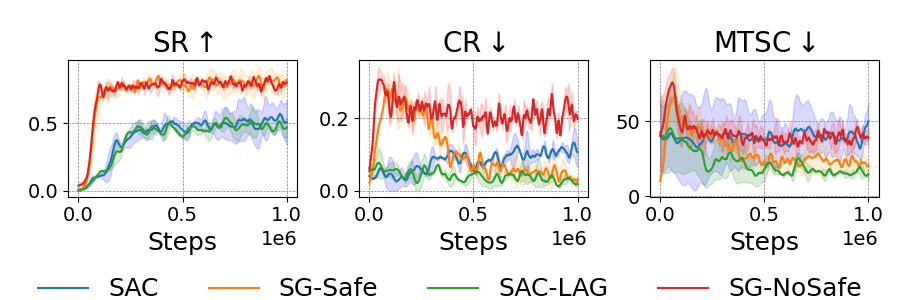
\includegraphics[width=0.9\textwidth]{RQ1_Point_Baselines.png}
\caption{Обучение SAC, SAC-LAG, SG-NoSafe и SG-Safe в среде Safety Gym Point. Показаны доля успешных эпизодов (SR), MTSC ($C(\pi)$), частота столкновений (CR) и число взаимодействий со средой. Результаты усреднены по трём запускам.}
    \label{fig:sgsafe_training_comparison}
\end{figure}

\subsection{Сравнение с методами, использующими априорную информацию}
\label{subsec:sgsafe_rq2}

В этом эксперименте SG-Safe сравнивался с методами, которым требуется дополнительная информация о среде. Основной пример такого подхода~--- L-RRT. В отличие от SG-Safe, этот метод предполагает полную наблюдаемость состояния и использует RRT*-планирование во время исполнения.

Результаты в табл.~\ref{tab:sgsafe_polamp_l1}--\ref{tab:sgsafe_polamp_avg} показывают, что SG-Safe достигает меньшего значения MTSC, хотя работает только с частичным наблюдением. L-RRT может строить геометрически допустимые траектории, но это не всегда приводит к более безопасному поведению при исполнении. Такие траектории могут быть длиннее и проходить рядом с областями ограничений. Кроме того, Lyapunov-контроллер, который отслеживает построенный путь, сам по себе не учитывает препятствия. Поэтому даже формально безопасный маршрут может приводить к рискованным действиям на этапе движения агента.

Отдельно была проверена устойчивость методов при увеличении числа препятствий. В эксперименте плотность препятствий изменялась от $N_{\mathrm{obs}}=2$ до $N_{\mathrm{obs}}=10$. Как показано на рис.~\ref{fig:sgsafe_lrrt_obstacle_density}, SG-Safe сохраняет устойчивое поведение при росте сложности среды и не допускает столкновений вплоть до шести препятствий. L-RRT начинает заметно ухудшаться уже при четырёх препятствиях. При $8$--$10$ препятствиях это различие становится сильнее: SG-Safe чаще достигает цели, тогда как L-RRT испытывает трудности с построением допустимой траектории через узкие безопасные области.

Результаты в табл.~\ref{tab:sgsafe_classic_planners} показывают различие между планировщиками более детально. RRT с управлением Дубинса может давать высокую долю успешных эпизодов, но его траектории проходят близко к препятствиям и используют только кинематическое управление $(v,\gamma)$. В L-RRT дополнительно возникает проблема отслеживания траектории в узких коридорах: промежуточные точки могут быть геометрически допустимыми, но труднодостижимыми для контроллера. В таких случаях агент либо сталкивается с препятствием, либо останавливается из-за блокировки следующего действия защитным фильтром.

SG-Safe устроен иначе. Он не строит отдельную траекторию во время исполнения, а сразу выдаёт кинодинамически допустимое действие $(a,\omega)$ обученной стратегией. Поэтому на этапе применения метод не тратит время на планирование и работает примерно в $10$ раз быстрее, сохраняя конкурентную долю успешных эпизодов и лучшее время достижения цели. Рис.~\ref{fig:sgsafe_lrrt_trajectories} показывает типичные ошибки L-RRT в коридорных задачах и иллюстрирует, почему отсутствие отдельного планировщика во время исполнения может быть преимуществом для SG-Safe.

SG-Safe требует дополнительных вычислений на этапе обучения, поскольку оптимизирует дополнительную стратегию генерации подцелей (формула~\ref{eq:sgsafe_safe_policy_improvement}) вместе со стандартными обновлениями безопасного актор-критика по мини-пакетам из буфера воспроизведения опыта. Однако эти дополнительные затраты ограничены этапом обучения и не влияют на применение метода. На этапе исполнения стратегия генерации подцелей отбрасывается, и используется только обученная безопасная низкоуровневая стратегия. Поэтому вычисление действия на каждом шаге сводится к одному прямому проходу через актор, что сопоставимо с SAC-LAG. В отличие от этого, методы на основе планирования дополнительно требуют затрат на планирование и отслеживание траектории во время исполнения, например ненулевого времени планирования в табл.~\ref{tab:sgsafe_classic_planners}, чего предложенный метод избегает на этапе применения.

\begin{figure}[t]
\centering
\begin{minipage}[t]{0.49\linewidth}
  \centering
  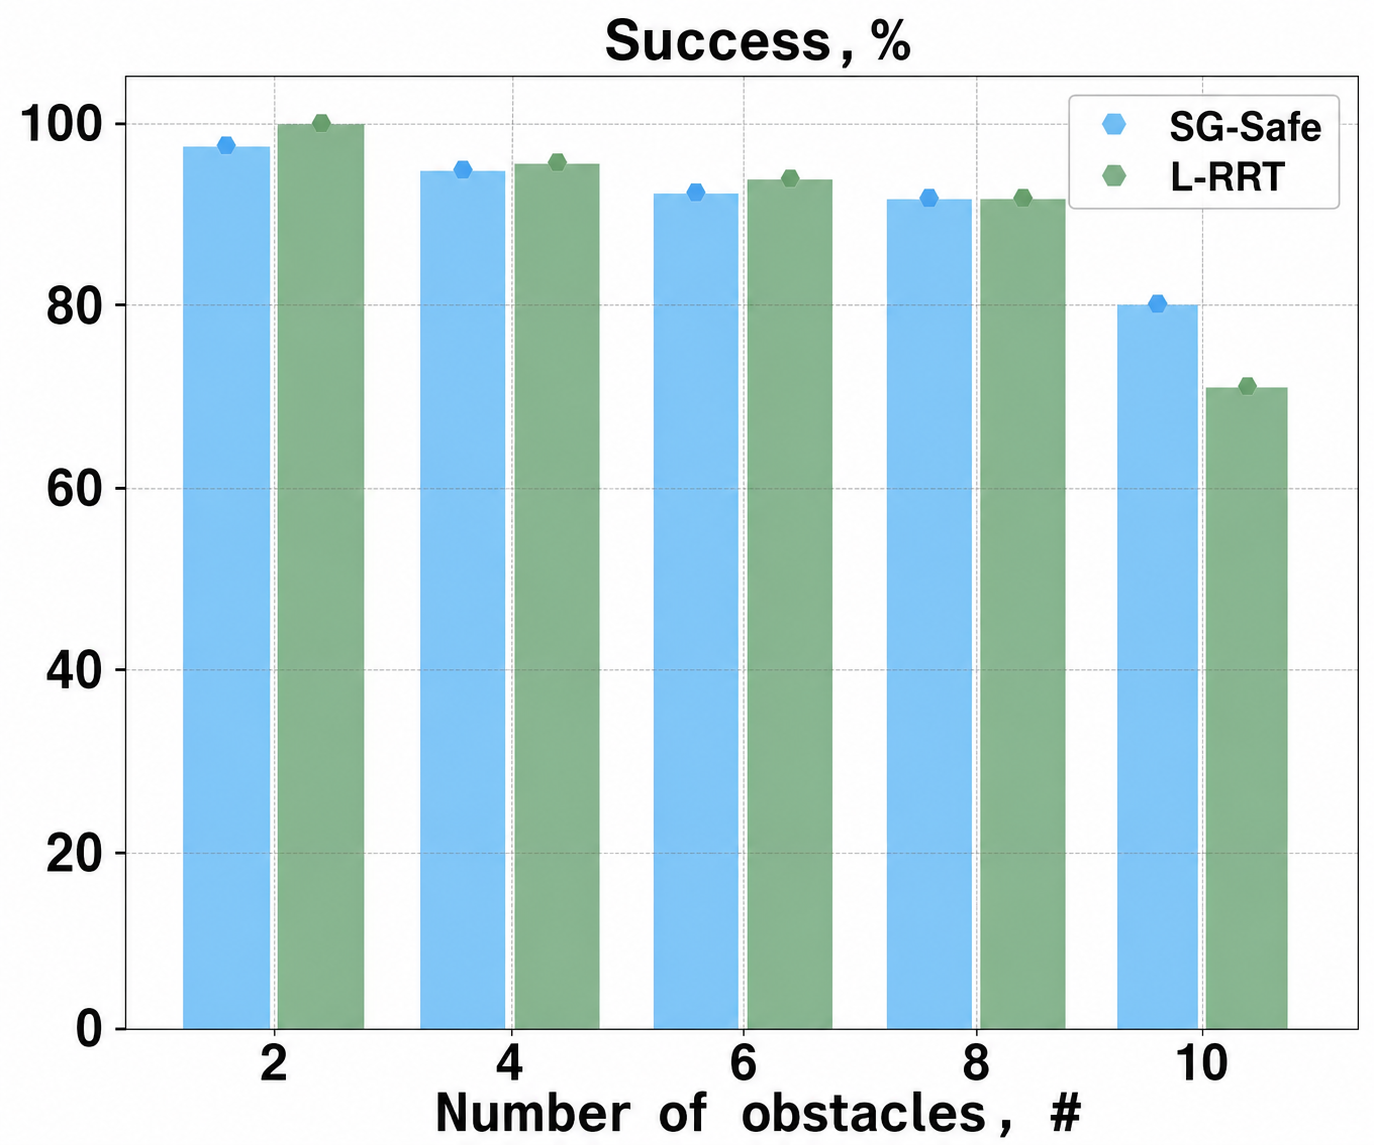
\includegraphics[height=0.22\textheight,keepaspectratio]{lyap_hist_1_edited.png}
\end{minipage}\hfill
\begin{minipage}[t]{0.49\linewidth}
  \centering
  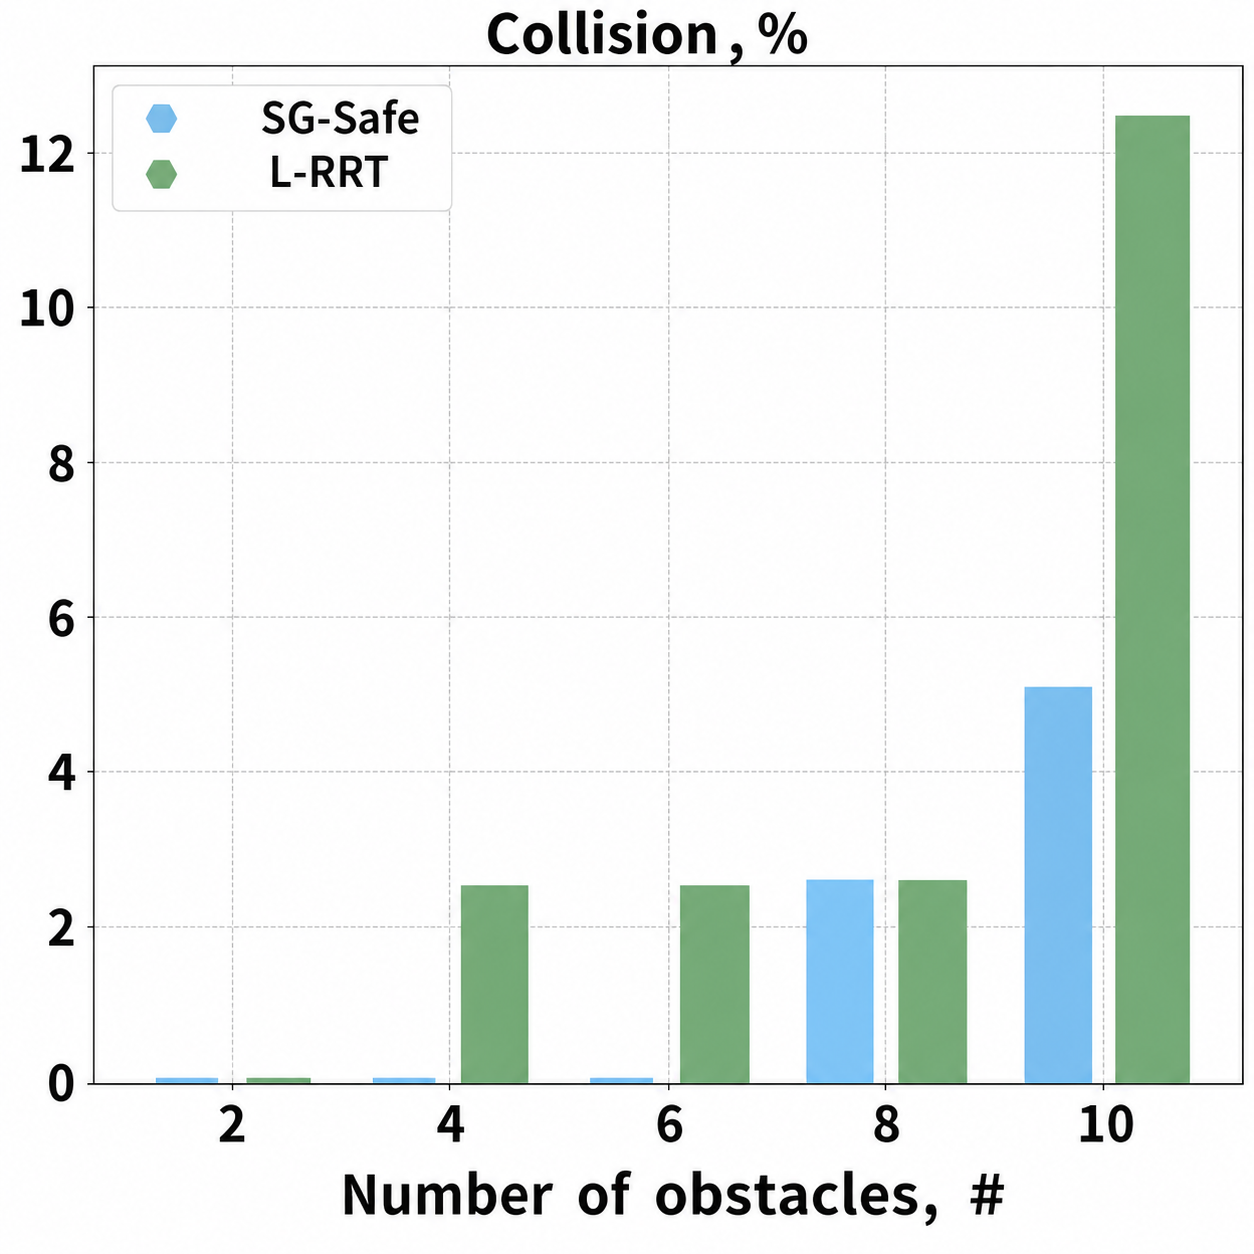
\includegraphics[height=0.22\textheight,keepaspectratio]{lyap_hist_2_edited.png}
\end{minipage}
\caption{Сравнение SG-Safe и Lyapunov RRT в Safety Gym Point при разном числе препятствий. \textbf{Слева} показана доля успешных эпизодов, \textbf{справа} --- частота столкновений. Результаты усреднены по трём запускам.}
\label{fig:sgsafe_lrrt_obstacle_density}
\end{figure}

\begin{figure}[t]
\centering
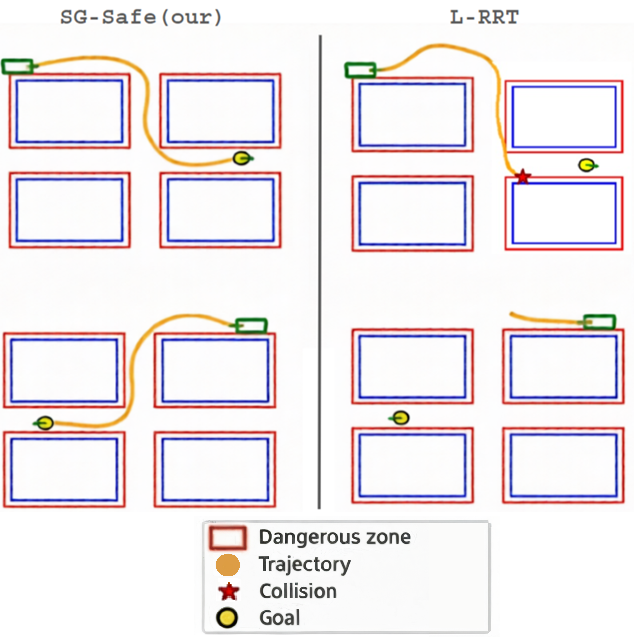
\includegraphics[width=0.78\linewidth]{SgSafeLRRT_compartion.png}
\caption{Примеры траекторий SG-Safe и L-RRT в задачах POLAMP.}
\label{fig:sgsafe_lrrt_trajectories}
\end{figure}

\subsection{Сравнение с базовыми методами}
\label{subsec:sgsafe_rq3}

\paragraph{Бенчмарк Safety Gym.}
В табл.~\ref{tab:sgsafe_sg_point_car}--\ref{tab:sgsafe_sg_avg} приведены результаты на Safety Gym. Среди обучаемых методов SG-Safe достигает наименьшей средней частоты столкновений ($CR=0.03$, табл.~\ref{tab:sgsafe_sg_avg}), сохраняя высокую долю успешных эпизодов ($SR=0.87$). SAC-LAG достигает немного меньшего значения MTSC, однако это в основном связано с чрезмерно консервативным поведением: стратегия часто остаётся неподвижной, что снижает воздействие опасных зон, но ухудшает выполнение задачи. В отличие от SAC-LAG, SG-Safe сохраняет направленное к цели поведение и снижает число столкновений за счёт остановки на безопасном расстоянии от опасных зон. Также наблюдается, что SG-Safe может превосходить SG-NoSafe на некоторых задачах, например Point и Doggo, что показывает: явная оптимизация безопасности может повышать эффективность исследования за счёт предотвращения небезопасных обходных траекторий и повторного восстановления после нарушений.

\begin{table}[ht!]
\centering
\caption{Результаты на Safety Gym Point и Car. Значения --- среднее по трём случайным запускам. SR --- доля успешных эпизодов, CR --- частота столкновений, MTSC --- Mean Total Safety Cost, средний накопленный штраф безопасности за эпизод ($C(\pi)$); меньше --- лучше для CR и MTSC. Жирным выделены лучшие значения в каждой среде; красным --- методы с полной наблюдаемостью.}
\label{tab:sgsafe_sg_point_car}
\small
\setlength{\tabcolsep}{4pt}
\renewcommand{\arraystretch}{1.08}
\begin{tabularx}{0.72\linewidth}{@{}>{\raggedright\arraybackslash}X>{\centering\arraybackslash}p{0.14\linewidth}>{\centering\arraybackslash}p{0.14\linewidth}>{\centering\arraybackslash}p{0.16\linewidth}@{}}
Strategy & SR$\uparrow$ & CR$\downarrow$ & MTSC$\downarrow$ \\
\hline \hline
\multicolumn{4}{@{}l}{\textit{Point}} \\
SG-Safe (ours) & 0.93 & \textbf{0.02} & 20.7 \\
SG-NoSafe & 0.89 & 0.11 & 33.2 \\
\rowcolor{red!10} L-RRT & \textbf{1} & 0.00 & 42.2 \\
SAC-LAG & 0.54 & 0.04 & \textbf{13.4} \\
SAC & 0.61 & 0.12 & 26.3 \\
CPO & 0.60 & 0.28 & 146.1 \\
\hline
\multicolumn{4}{@{}l}{\textit{Car}} \\
SG-Safe (ours) & 0.75 & \textbf{0.05} & 20.7 \\
SG-NoSafe & 0.76 & 0.24 & 33.4 \\
\rowcolor{red!10} L-RRT & \textbf{0.95} & \textbf{0.05} & 37.6 \\
SAC-LAG & 0.56 & \textbf{0.04} & \textbf{13.8} \\
SAC & 0.30 & 0.78 & 17.3 \\
CPO & 0.62 & 0.33 & 133.6 \\
\hline \hline
\end{tabularx}
\end{table}

\begin{table}[ht!]
\centering
\caption{Результаты на Safety Gym Doggo и Sweeps. Обозначения метрик --- см. табл.~\ref{tab:sgsafe_sg_point_car}.}
\label{tab:sgsafe_sg_doggo_sweeps}
\small
\setlength{\tabcolsep}{4pt}
\renewcommand{\arraystretch}{1.08}
\begin{tabularx}{0.72\linewidth}{@{}>{\raggedright\arraybackslash}X>{\centering\arraybackslash}p{0.14\linewidth}>{\centering\arraybackslash}p{0.14\linewidth}>{\centering\arraybackslash}p{0.16\linewidth}@{}}
Strategy & SR$\uparrow$ & CR$\downarrow$ & MTSC$\downarrow$ \\
\hline \hline
\multicolumn{4}{@{}l}{\textit{Doggo}} \\
SG-Safe (ours) & 0.79 & \textbf{0.05} & \textbf{12.5} \\
SG-NoSafe & 0.74 & 0.20 & 40.2 \\
\rowcolor{red!10} L-RRT & \textbf{0.93} & 0.08 & 17.1 \\
SAC-LAG & 0.02 & 0.10 & 22.6 \\
SAC & 0.08 & 0.15 & 44.63 \\
CPO & 0.65 & 0.30 & 86.8 \\
\hline
\multicolumn{4}{@{}l}{\textit{Sweeps}} \\
SG-Safe (ours) & \textbf{1} & \textbf{0} & \textbf{0.98} \\
SG-NoSafe & \textbf{1} & \textbf{0} & 12.87 \\
\rowcolor{red!10} L-RRT & \textbf{1} & \textbf{0} & 9.0 \\
SAC-LAG & 0.47 & \textbf{0} & 1.25 \\
SAC & 0.55 & 0.05 & 5.16 \\
CPO & 0.15 & 0.85 & 102 \\
\hline \hline
\end{tabularx}
\end{table}

\begin{table}[ht!]
\centering
\caption{Усреднённые результаты на Safety Gym (Avg.) по средам Point, Car, Doggo и Sweeps. Обозначения метрик --- см. табл.~\ref{tab:sgsafe_sg_point_car}.}
\label{tab:sgsafe_sg_avg}
\small
\setlength{\tabcolsep}{4pt}
\renewcommand{\arraystretch}{1.08}
\begin{tabularx}{0.72\linewidth}{@{}>{\raggedright\arraybackslash}X>{\centering\arraybackslash}p{0.14\linewidth}>{\centering\arraybackslash}p{0.14\linewidth}>{\centering\arraybackslash}p{0.16\linewidth}@{}}
Strategy & SR$\uparrow$ & CR$\downarrow$ & MTSC$\downarrow$ \\
\hline \hline
SG-Safe (ours) & 0.87 & \textbf{0.03} & \textbf{13.7} \\
SG-NoSafe & 0.85 & 0.14 & 29.9 \\
\rowcolor{red!10} L-RRT & \textbf{0.97} & 0.03 & 26.5 \\
SAC-LAG & 0.40 & \textbf{0.05} & 12.8 \\
SAC & 0.39 & 0.28 & 23.3 \\
CPO & 0.51 & 0.44 & 117.1 \\
\hline \hline
\end{tabularx}
\end{table}

\paragraph{Бенчмарк POLAMP.}
Результаты на POLAMP приведены в табл.~\ref{tab:sgsafe_polamp_l1}--\ref{tab:sgsafe_polamp_avg} и табл.~\ref{tab:sgsafe_classic_planners}. Наиболее сложной является постановка Level~2, где агенту требуется проходить длинные маршруты при частичной наблюдаемости и наличии препятствий. В этой группе задач SG-Safe достигает доли успешных эпизодов ($SR = 0.897$), тогда как у одноуровневых базовых методов значения находятся в диапазоне $0$--$0.363$. При этом метод сохраняет низкое значение MTSC. Такой результат показывает, что подцели в SG-Safe не просто ускоряют обучение, а помогают агенту находить траектории, которые одноуровневая стратегия с ограничениями обычно не обнаруживает.

В сравнение также включён ADVICE как метод, использующий дополнительную информацию для фильтрации действий. В POLAMP он показывает почти нулевую долю успешных эпизодов. Одна из причин состоит в том, что метод основан на DDPG и не использует переопределение целей в стиле HER, что особенно важно в задачах с большим горизонтом и разреженной наградой. Поэтому для SAC-подобных базовых методов в данной работе используется HER, чтобы сравнение было устойчивым и не сводилось только к проблеме редкого обучающего сигнала.

Методы с фильтрацией действий во время исполнения, например SAC-RCBF, требуют дополнительных предположений о модели робота или функции штрафов и несут вычислительные затраты на этапе выбора действия. Одноуровневые методы, такие как SAC и SAC-LAG, в Level~2 также оказываются недостаточными: штрафы ограничивает исследование, но не даёт механизма, который направлял бы агента через длинную последовательность промежуточных состояний.

\begin{table}[ht!]
\centering
\caption{Результаты на POLAMP Level~1 с указанием неопределённости. Каждая метрика --- среднее $\pm$ стандартное отклонение; ниже указан 95\%-ный бутстрэп-доверительный интервал (CI95). SR --- доля успешных эпизодов, CR --- частота столкновений, MTSC --- Mean Total Safety Cost, средний накопленный штраф безопасности за эпизод. Красным выделены методы с привилегированной информацией и/или явными моделями.}
\label{tab:sgsafe_polamp_l1}
\footnotesize
\setlength{\tabcolsep}{3pt}
\renewcommand{\arraystretch}{1.05}
\begin{tabularx}{0.85\linewidth}{@{}>{\raggedright\arraybackslash}X>{\centering\arraybackslash}p{0.22\linewidth}>{\centering\arraybackslash}p{0.22\linewidth}>{\centering\arraybackslash}p{0.22\linewidth}@{}}
Strategy & SR$\uparrow$ & CR$\downarrow$ & MTSC$\downarrow$ \\
\hline \hline
SG-Safe (ours) & \textbf{0.919$\pm$0.009} & \textbf{0.025$\pm$0.012} & 1.567$\pm$0.331 \\
 & \scriptsize CI95 [0.913, 0.925] & \scriptsize CI95 [0.017, 0.033] & \scriptsize CI95 [1.288, 1.838] \\
SAC-LAG & 0.727$\pm$0.011 & 0.029$\pm$0.009 & 6.765$\pm$2.954 \\
 & \scriptsize CI95 [0.717, 0.735] & \scriptsize CI95 [0.023, 0.035] & \scriptsize CI95 [5.069, 9.456] \\
SAC & 0.610$\pm$0.040 & 0.023$\pm$0.014 & 11.252$\pm$3.718 \\
 & \scriptsize CI95 [0.579, 0.642] & \scriptsize CI95 [0.010, 0.031] & \scriptsize CI95 [8.221, 14.002] \\
SAC-NCMP & 0.427$\pm$0.000 & 0.573$\pm$0.000 & \textbf{0.869$\pm$0.015} \\
 & \scriptsize CI95 [0.427, 0.427] & \scriptsize CI95 [0.573, 0.573] & \scriptsize CI95 [0.856, 0.880] \\
\rowcolor{red!10} SAC-RCBF & 0.344$\pm$0.032 & 0.240$\pm$0.025 & 4.456$\pm$3.076 \\
\rowcolor{red!10} & \scriptsize CI95 [0.320, 0.368] & \scriptsize CI95 [0.220, 0.256] & \scriptsize CI95 [2.236, 6.834] \\
ADVICE & 0.000$\pm$0.000 & 0.031$\pm$0.000 & 0.031$\pm$0.000 \\
 & \scriptsize CI95 [0.000, 0.000] & \scriptsize CI95 [0.031, 0.031] & \scriptsize CI95 [0.031, 0.031] \\
\rowcolor{red!10} L-RRT & 0.551$\pm$0.152 & 0.350$\pm$0.028 & 8.335$\pm$1.898 \\
\rowcolor{red!10} & \scriptsize CI95 [0.444, 0.672] & \scriptsize CI95 [0.331, 0.373] & \scriptsize CI95 [6.996, 9.990] \\
\hline \hline
\end{tabularx}
\end{table}

\begin{table}[ht!]
\centering
\caption{Результаты на POLAMP Level~2 с указанием неопределённости. Обозначения метрик --- см. табл.~\ref{tab:sgsafe_polamp_l1}.}
\label{tab:sgsafe_polamp_l2}
\footnotesize
\setlength{\tabcolsep}{3pt}
\renewcommand{\arraystretch}{1.05}
\begin{tabularx}{0.85\linewidth}{@{}>{\raggedright\arraybackslash}X>{\centering\arraybackslash}p{0.22\linewidth}>{\centering\arraybackslash}p{0.22\linewidth}>{\centering\arraybackslash}p{0.22\linewidth}@{}}
Strategy & SR$\uparrow$ & CR$\downarrow$ & MTSC$\downarrow$ \\
\hline \hline
SG-Safe (ours) & \textbf{0.875$\pm$0.052} & \textbf{0.031$\pm$0.017} & 5.103$\pm$2.632 \\
 & \scriptsize CI95 [0.843, 0.915] & \scriptsize CI95 [0.018, 0.044] & \scriptsize CI95 [2.838, 6.981] \\
SAC-LAG & 0.000$\pm$0.000 & \textbf{0.004$\pm$0.006} & 1.319$\pm$0.802 \\
 & \scriptsize CI95 [0.000, 0.000] & \scriptsize CI95 [0.000, 0.008] & \scriptsize CI95 [0.763, 2.004] \\
SAC & 0.000$\pm$0.000 & 0.010$\pm$0.015 & 5.054$\pm$2.325 \\
 & \scriptsize CI95 [0.000, 0.000] & \scriptsize CI95 [0.000, 0.023] & \scriptsize CI95 [3.340, 7.035] \\
SAC-NCMP & 0.000$\pm$0.000 & 1.000$\pm$0.000 & 1.369$\pm$0.020 \\
 & \scriptsize CI95 [0.000, 0.000] & \scriptsize CI95 [1.000, 1.000] & \scriptsize CI95 [1.350, 1.383] \\
\rowcolor{red!10} SAC-RCBF & 0.008$\pm$0.010 & 0.050$\pm$0.025 & 8.625$\pm$1.823 \\
\rowcolor{red!10} & \scriptsize CI95 [0.000, 0.015] & \scriptsize CI95 [0.030, 0.070] & \scriptsize CI95 [7.188, 10.133] \\
ADVICE & 0.000$\pm$0.000 & 0.010$\pm$0.000 & \textbf{0.010$\pm$0.000} \\
 & \scriptsize CI95 [0.000, 0.000] & \scriptsize CI95 [0.010, 0.010] & \scriptsize CI95 [0.010, 0.010] \\
\rowcolor{red!10} L-RRT & 0.125$\pm$0.050 & 0.664$\pm$0.165 & 12.154$\pm$4.167 \\
\rowcolor{red!10} & \scriptsize CI95 [0.089, 0.160] & \scriptsize CI95 [0.547, 0.780] & \scriptsize CI95 [9.208, 15.100] \\
\hline \hline
\end{tabularx}
\end{table}

\begin{table}[ht!]
\centering
\caption{Усреднённые результаты на POLAMP (Avg.) по Level~1 и Level~2 с указанием неопределённости. Обозначения метрик --- см. табл.~\ref{tab:sgsafe_polamp_l1}.}
\label{tab:sgsafe_polamp_avg}
\footnotesize
\setlength{\tabcolsep}{3pt}
\renewcommand{\arraystretch}{1.05}
\begin{tabularx}{0.85\linewidth}{@{}>{\raggedright\arraybackslash}X>{\centering\arraybackslash}p{0.22\linewidth}>{\centering\arraybackslash}p{0.22\linewidth}>{\centering\arraybackslash}p{0.22\linewidth}@{}}
Strategy & SR$\uparrow$ & CR$\downarrow$ & MTSC$\downarrow$ \\
\hline \hline
SG-Safe (ours) & \textbf{0.897$\pm$0.026} & 0.028$\pm$0.010 & 3.335$\pm$1.327 \\
 & \scriptsize CI95 [0.878, 0.920] & \scriptsize CI95 [0.017, 0.039] & \scriptsize CI95 [2.063, 4.409] \\
SAC-LAG & 0.364$\pm$0.006 & \textbf{0.017$\pm$0.005} & 4.042$\pm$1.530 \\
 & \scriptsize CI95 [0.358, 0.368] & \scriptsize CI95 [0.012, 0.022] & \scriptsize CI95 [2.916, 5.730] \\
SAC & 0.305$\pm$0.020 & \textbf{0.017$\pm$0.010} & 8.153$\pm$2.192 \\
 & \scriptsize CI95 [0.290, 0.321] & \scriptsize CI95 [0.005, 0.027] & \scriptsize CI95 [5.780, 10.519] \\
SAC-NCMP & 0.214$\pm$0.000 & 0.787$\pm$0.000 & 1.119$\pm$0.012 \\
 & \scriptsize CI95 [0.214, 0.214] & \scriptsize CI95 [0.787, 0.787] & \scriptsize CI95 [1.103, 1.131] \\
\rowcolor{red!10} SAC-RCBF & 0.176$\pm$0.017 & 0.145$\pm$0.017 & 6.541$\pm$1.788 \\
\rowcolor{red!10} & \scriptsize CI95 [0.160, 0.192] & \scriptsize CI95 [0.125, 0.163] & \scriptsize CI95 [4.712, 8.483] \\
ADVICE & 0.000$\pm$0.000 & 0.021$\pm$0.000 & \textbf{0.021$\pm$0.000} \\
 & \scriptsize CI95 [0.000, 0.000] & \scriptsize CI95 [0.021, 0.021] & \scriptsize CI95 [0.021, 0.021] \\
\rowcolor{red!10} L-RRT & 0.338$\pm$0.080 & 0.507$\pm$0.084 & 10.245$\pm$2.289 \\
\rowcolor{red!10} & \scriptsize CI95 [0.267, 0.416] & \scriptsize CI95 [0.439, 0.576] & \scriptsize CI95 [8.102, 12.545] \\
\hline \hline
\end{tabularx}
\end{table}

\begin{table}[ht!]
\centering
\caption{Результаты экспериментов на средах POLAMP с классическими планировщиками. TTR --- время достижения цели в шагах среды, PT --- время планирования в секундах, ET --- время исполнения в секундах. Базовые методы, выделенные красным, используют полную информацию о состоянии, включая точные положения препятствий и геометрию робота.}
\label{tab:sgsafe_classic_planners}
\small
\setlength{\tabcolsep}{3pt}
\renewcommand{\arraystretch}{1.05}
\begin{tabularx}{\linewidth}{@{}>{\raggedright\arraybackslash}X>{\centering\arraybackslash}p{0.07\linewidth}>{\centering\arraybackslash}p{0.07\linewidth}>{\centering\arraybackslash}p{0.08\linewidth}>{\centering\arraybackslash}p{0.09\linewidth}>{\centering\arraybackslash}p{0.08\linewidth}>{\centering\arraybackslash}p{0.09\linewidth}@{}}
Strategy & SR$\uparrow$ & CR$\downarrow$ & MTSC$\downarrow$ & TTR$\downarrow$, t & PT$\downarrow$, s & ET$\downarrow$, s \\
\hline \hline
\multicolumn{7}{@{}l}{\textit{Level 1}} \\
SG-Safe (ours) & 0.92 & 0.03 & \textbf{1.57} & \textbf{47.52} & \textbf{0} & $9\cdot 10^{-3}$ \\
\rowcolor{red!10} L-RRT & 0.55 & 0.35 & 8.34 & 104.2 & 10.4 & $9\cdot 10^{-3}$ \\
\rowcolor{red!10} RRT & \textbf{1} & 0 & 2.1 & 86.3 & 18.3 & -- \\
\hline
\multicolumn{7}{@{}l}{\textit{Level 2}} \\
SG-Safe (ours) & 0.88 & 0.03 & \textbf{5.10} & 164.53 & \textbf{0} & $9.3\cdot 10^{-3}$ \\
\rowcolor{red!10} L-RRT & 0.12 & 0.66 & 12.15 & 170.1 & 30.2 & $9.2\cdot 10^{-3}$ \\
\rowcolor{red!10} RRT & \textbf{1} & 0 & 9 & \textbf{111.4} & 51.4 & -- \\
\hline \hline
\end{tabularx}
\end{table}

Разброс между случайными запусками связан главным образом со стохастической инициализацией сетей, выборкой мини-пакетов из replay buffer и шумом исследования. В Safety Gym дополнительный вклад дают случайные начальные положения целей и опасных зон. POLAMP устроен более детерминированно, поэтому там вариативность результатов в большей степени определяется самим процессом оптимизации.

В целом SG-Safe достигает лучшего баланса между безопасностью и эффективностью на обоих бенчмарках среди сквозных методов обучения с подкреплением, сохраняя применимость в рассматриваемой постановке с частичной наблюдаемостью и ограниченной информацией о среде.

\subsection{Анализ компонент метода}
\label{subsec:sgsafe_rq4}

\paragraph{Анализ архитектуры критика штрафов.}

Был исследован алгоритм SG-Safe с архитектурами, использующими один и два критика штрафов $Q_c^{\pi_{\theta}}$. Для проверки устойчивости результатов при разных конфигурациях были проведены эксперименты в среде Safety Gym с двумя роботами: Point и Car. В существующей литературе встречаются реализации как с одним критиком~\cite{hogewind2022safe}, так и с двумя критиками~\cite{chow2017risk}, однако сравнительный анализ этих архитектур ранее не проводился.

Результаты, приведённые на рис.~\ref{fig:cost_critic_compartion}, показывают, что использование одного критика штрафов приводит к переоценке накопленных штрафов $C(\pi)$. В результате алгоритм становится более консервативным и сильнее приоритизирует безопасность в ущерб эффективности решения задачи. Сходное осторожное поведение наблюдается при выборе максимального значения между двумя критиками штрафов: завышенные оценки штрафов смещают стратегию в сторону более консервативных решений. Напротив, использование двух критиков и выбор минимального значения приводит к менее ограниченному поведению и повышает эффективность решения задачи, хотя общая безопасность при этом снижается.

По результатам этого сравнения в SG-Safe используется вариант с двумя критиками штрафов и минимальной агрегацией их оценок. Такая конфигурация не даёт самой осторожной оценки штрафов, но в проведённых экспериментах она лучше сохраняет способность агента решать задачу. При этом значение накопленных штрафов остаётся в допустимых пределах, заданных бюджетом ($d$). Поэтому дальнейшие эксперименты проводятся именно с этой архитектурой критика штрафов.

\begin{figure}[ht!]
\centering
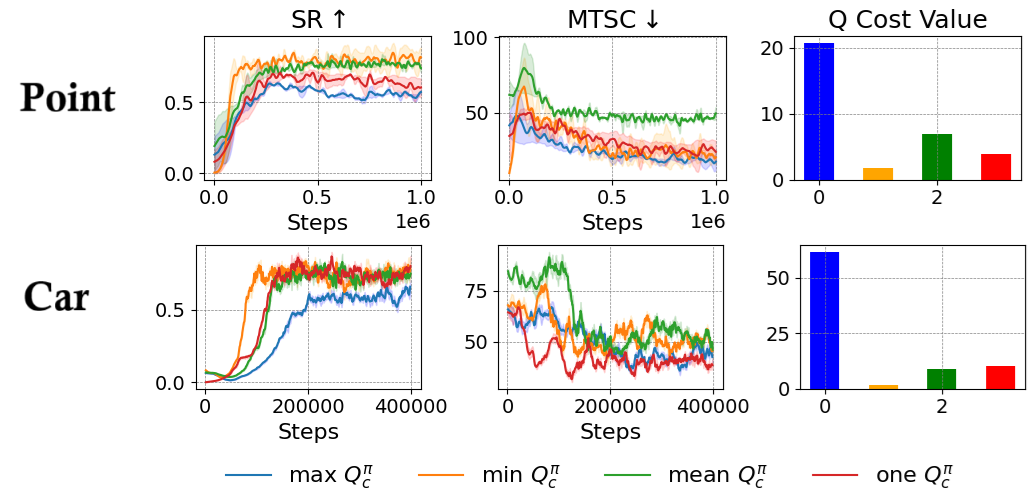
\includegraphics[width=0.9\textwidth]{RQ3_Ablation_QCost.png}
\caption{Влияние числа критиков штрафов ($Q^{\pi_\theta}_c$) на обучение SG-Safe в средах Safety Gym Point и Safety Gym Car. Показаны доля успешных эпизодов (SR), MTSC ($C(\pi)$), итоговая оценка критика штрафов и число взаимодействий со средой. Результаты усреднены по трём запускам.}
\label{fig:cost_critic_compartion}
\end{figure}

\paragraph{Анализ чувствительности к гиперпараметрам.}

Дополнительно были проведены абляционные эксперименты по трём параметрам метода: весу влияния подцелей ($\alpha$), начальному значению множителя Лагранжа ($\lambda_0$) и бюджету штрафов ($d$) (рис.~\ref{fig:hyperparams_ablation}).

Наиболее заметный эффект даёт параметр $\alpha$. При $\alpha = 1.0$ подцели начинают слишком сильно влиять на обновление стратегии, и обучение становится неустойчивым: доля успешных эпизодов снижается до $0.2$. Это связано с тремя факторами: 1) низким качеством начальных предсказаний подцелей на ранних этапах обучения, 2) наличием задач, которые могут быть решены без использования подцелей, и 3) принудительным следованием неточным подцелям, что приводит к попаданию в локальные оптимумы.

\begin{figure}[ht!]
\centering
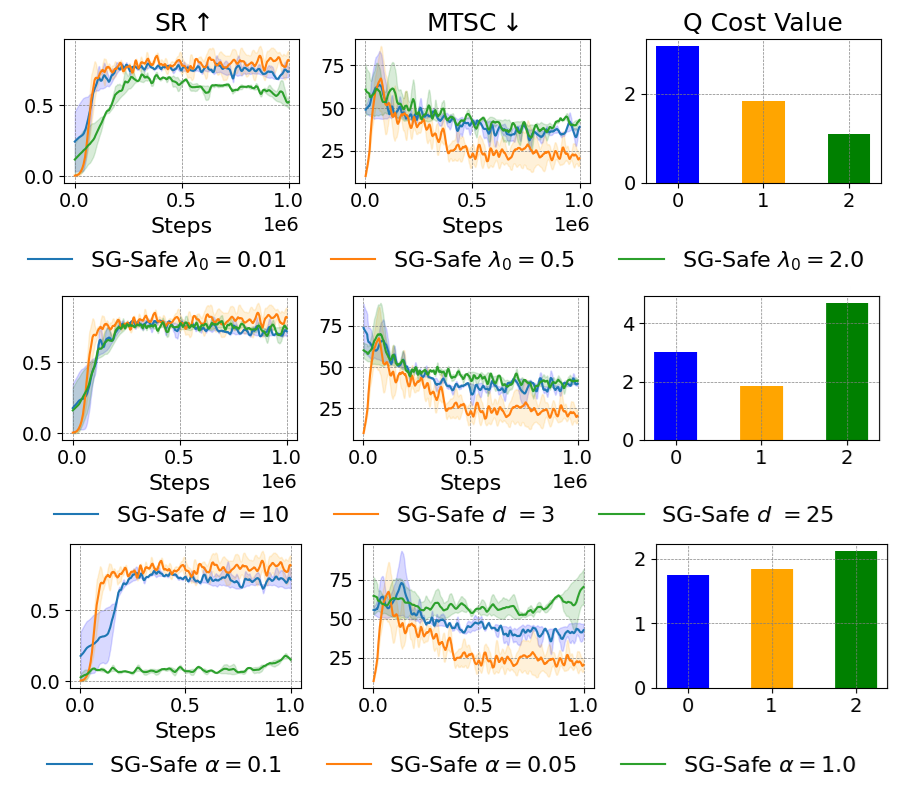
\includegraphics[width=0.9\textwidth]{RQ3_Ablation_Hyperparams.png}
\caption{Исследование гиперпараметров алгоритма SG-Safe: начального значения множителя Лагранжа $\lambda_0$, бюджета штрафов $d$ и коэффициента $\alpha$ в среде Safety Gym Point. SR --- доля успешных эпизодов, MTSC --- Mean Total Safety Cost, средний накопленный штраф безопасности за эпизод ($C(\pi)$). Эксперименты проводились по трём случайным запускам.}
\label{fig:hyperparams_ablation}
\end{figure}

\noindent\textbf{Основные выводы анализа компонент метода:}
\begin{itemize}
\item \textbf{Критики штрафов}: два критика с выбором минимального значения обеспечивают наилучший баланс между безопасностью и эффективностью.
\item \textbf{Влияние подцелей} ($\alpha$): меньшие значения ($\alpha<1.0$) предотвращают срыв обучения.
\item \textbf{Коэффициент безопасности} ($\lambda_0$): умеренная инициализация позволяет эффективно обучать ограничения безопасности.
\item \textbf{Бюджет штрафов} ($d$): более строгие ограничения повышают безопасность, но снижают эффективность решения задачи.
\end{itemize}

\section{Выводы по главе}
\label{sec:sgsafe_conclusion}

В данной главе был представлен метод SG-Safe, направленный на повышение исследовательской способности безопасных стратегий в задачах с большим горизонтом. Метод использует стратегию генерации подцелей на этапе обучения: подцели не являются жёсткими командами, а выступают как дополнительный обучающий сигнал, смещающий безопасную стратегию к более информативным областям пространства состояний. На этапе исполнения используется только обученная безопасная стратегия, поэтому SG-Safe не требует дополнительного планирования во время применения.

Экспериментальные результаты показывают, что SG-Safe улучшает баланс между достижением цели и безопасностью по сравнению с другими методами безопасного обучения с подкреплением. На Safety Gym метод достигает среднего значения SR $0.87$ при CR $0.03$. Наиболее выраженный эффект наблюдается на POLAMP, где задачи имеют больший горизонт и требуют прохождения сложных коридорных маршрутов. На уровне Level~2 безопасные стратегии фактически не решают задачу: SAC-LAG и SAC достигают SR $0$, а другие базовые методы также показывают низкую успешность. В этих условиях SG-Safe достигает ($SR = 0.875$) при ($CR = 0.031$). Такой результат показывает, что подцели помогают безопасной стратегии не останавливаться в локальном поведении и продолжать поиск траекторий к цели. В среднем по POLAMP метод достигает ($SR = 0.897$) при ($CR = 0.028$).

По сравнению с L-RRT метод использует меньше априорной информации: он работает при частичной наблюдаемости и не строит отдельный план во время исполнения. Это особенно заметно на POLAMP Level~2. L-RRT имеет доступ к полной информации о среде, но достигает только ($SR = 0.125$) при ($CR = 0.664$). SG-Safe, напротив, сохраняет высокую успешность и низкую частоту столкновений без доступа к полной карте среды.

Эти результаты показывают, что генерация подцелей помогает закрыть слабое место одноуровневых безопасных стратегий~--- недостаточное исследование в задачах большого горизонта. При этом важно отметить ограничение метода: безопасность подцелей не задаётся отдельным формальным условием. Она возникает в результате обучения и согласования с распределением достижимых состояний, поэтому не является строгой гарантией. Поэтому следующий шаг состоит в контроле безопасности непосредственно на уровне выбора подцелей и на уровне исполнения действий, что рассматривается в следующей главе.
